\documentclass[11pt]{article}
\usepackage{amsmath, amssymb}
\usepackage{graphicx}
\usepackage{hyperref}
\usepackage[margin=1in]{geometry}
\usepackage[colorinlist,textsize=footnotesize]{todonotes}

\title{Design, Kinematics, and Control of a Two-Motor 5-Bar Parallel Linkage}
\author{Tumin}
\date{\today}

\begin{document}
\maketitle

\begin{abstract}
This report documents the design, kinematic modeling, trajectory generation, dynamics derivation, and control validation of a planar 5-bar parallel linkage actuated by two proximal-joint servos. Forward and inverse kinematics are solved in closed form and verified numerically. A minimum-jerk joint-space trajectory generator and an iterative learning control (ILC) scheme are implemented and validated in simulation. The physical mechanism has been assembled; camera-based joint angle calibration and the resulting sim-to-real comparison have not yet been performed and are left as future work.
\end{abstract}

\section{Introduction}

The 5-bar linkage is a two-degree-of-freedom planar parallel mechanism formed by two actuated proximal cranks and two passive distal couplers meeting at a shared end-effector node \cite{gamble2020fivebar}. Compared to serial arms, it offers a rigid, low-inertia structure with both actuators grounded at the base, at the cost of a more involved kinematic solution and a workspace bounded by linkage singularities. This project builds a physical instance of the mechanism and the accompanying software stack: kinematics, trajectory generation, dynamics, an iterative learning controller, and ArUco-marker-based visual joint sensing for eventual real-hardware calibration.

\section{Mechanism Design}

\subsection{Kinematic Architecture}

The mechanism is defined by three link lengths, configured in \texttt{config.toml}:
\begin{itemize}
  \item Proximal (crank) length: $l = 150$~mm
  \item Distal (coupler) length: $r = 200$~mm
  \item Base length: $b = 120$~mm
\end{itemize}

\todo[inline]{Resolve base-length discrepancy: \texttt{config.toml} has $b=120$~mm, \texttt{specs/system.md} records pivot-to-pivot base as $150$~mm. Software currently runs on the \texttt{config.toml} value. Not reconciled yet.}

\subsection{Mass Properties}

Per-link centers of mass (from pivot axis) and measured weights, from \texttt{specs/system.md}:

\begin{center}
\begin{tabular}{lcc}
\hline
Link & COM from axis & Mass \\
\hline
Left/Right cranker & 75~mm & 133~g \\
Left/Right coupler  & 95~mm & 175~g \\
\hline
\end{tabular}
\end{center}

\subsection{Bill of Materials}

The physical build (full list in \texttt{specs/parts.md}) uses: 2$\times$ MG958 digital servos (proximal actuation), 1$\times$ Arduino UNO R3, 2020 T-slot aluminium extrusion frame, 608ZZ deep-groove ball bearings at each pivot, M8/M5/M3 fasteners, and 3D-printed brackets, end-caps, a coupler block, and a parallel gripper end-effector.

\section{Kinematics}

\subsection{Forward Kinematics}

Given crank angles $(\theta_1, \theta_2)$, the end-effector position is found by solving the loop-closure constraint that both distal links (length $r$) meet at the same point, starting from the two crank-tip positions (offset by $l$ from each base pivot). This yields a quadratic in the end-effector $y$-coordinate with, in general, two solutions (the two ``working modes'' of the mechanism), implemented in \texttt{src/fk.py}.

\subsection{Inverse Kinematics}

Given a target end-effector position $(x, y)$, each crank angle is recovered independently via a law-of-cosines triangle solution over the crank/coupler/target-distance triangle on that side (\texttt{src/ik.py}). The solver raises on two degenerate cases: the target coinciding with a motor's own pivot, and the target lying outside the reachable annulus for that side (i.e. $|l - r| \le d \le l + r$ violated).

\subsection{Forward/Inverse Consistency}

\texttt{notebooks/project.ipynb} numerically verifies $FK(IK(x)) = x$ over sampled points drawn from within the mechanism's workspace bounds. All sampled round-trips passed, confirming the two closed-form solvers are mutually consistent.

\subsection{Jacobian and Singularities}

The end-effector Jacobian $J = \partial(x,y)/\partial(\theta_1,\theta_2)$ is computed numerically via first-order finite differences of the forward kinematics map (\texttt{notebooks/analysis.ipynb}). Configurations where $\det(J) = 0$ correspond to kinematic singularities of the closed loop, consistent with the general theory of closed-loop-chain singularities \cite{gosselin1990singularity}. The same notebook was also used, in an exploratory capacity, to sweep candidate base/proximal/distal dimensions against reachable workspace area and required servo torque before the dimensions in \texttt{config.toml} were fixed; those sweep values do not represent the final build.

\todo[inline]{Once the base-length discrepancy above is resolved and final link lengths are locked, re-run \texttt{notebooks/analysis.ipynb}'s workspace/singularity/torque sweep against the final dimensions and fold the resulting plots into this section.}

\section{Trajectory Generation}

\subsection{Minimum-Jerk Profile}

Point-to-point joint motions use a quintic minimum-jerk time-scaling $s(t)$ on normalized time $t \in [0,1]$, with boundary conditions of zero velocity and acceleration at both ends. Minimizing $\int \dddot{x}(t)^2\,dt$ via calculus of variations yields (derivation in \texttt{notebooks/min\_jerk\_traj.ipynb}, matching the classical minimum-jerk model \cite{flash1985coordination}):
\begin{align}
s(t) &= 10t^3 - 15t^4 + 6t^5 \\
\dot{s}(t) &= 30t^2 - 60t^3 + 30t^4 \\
\ddot{s}(t) &= 60t - 180t^2 + 120t^3
\end{align}
implemented in \texttt{src/trajectory.py}. Each joint angle is interpolated as $\theta_i(t) = \theta_i^{start} + (\theta_i^{end}-\theta_i^{start})\,s(t)$.

\subsection{Multi-Waypoint Chaining}

\texttt{waypoint2traj} chains a list of joint-space waypoints into one continuous trajectory by concatenating per-segment minimum-jerk profiles, without duplicating shared junction points.

\todo[inline]{Define and report the final operating trajectory/waypoint set (workspace path the arm will actually run) once link lengths are finalized and the Section~2.1 base-length discrepancy is resolved -- current waypoints used in testing are exploratory, not the final task trajectory.}

\section{Dynamics}

The Lagrangian dynamics of the mechanism were derived symbolically in \texttt{notebooks/euler\_lagrange.ipynb} using SymPy. Center-of-mass positions and velocities were derived for all four moving links (two per side) as functions of $(\theta_1,\theta_2)$ and the passive coupler angles $(\phi_1,\phi_2)$, with $\dot\phi_i$ related to $(\dot\theta_1,\dot\theta_2)$ through the time-derivative of the loop-closure constraint. Because the mechanism is planar and mounted perpendicular to gravity, every link's center of mass stays at constant height regardless of $(\theta_1,\theta_2)$; potential energy is therefore constant and drops out of the Lagrangian, giving $L = T$. Applying the Euler-Lagrange equation
\[
\frac{d}{dt}\left(\frac{\partial T}{\partial \dot\theta_i}\right) - \frac{\partial T}{\partial \theta_i} = \tau_i
\]
yields closed-form symbolic expressions for the two actuator torques $\tau_1, \tau_2$, cached in \texttt{tau.pkl}.

The symbolic torque expressions are complete.

\todo[inline]{Numeric evaluation of $\tau_1,\tau_2$ against the mechanism's real link masses/lengths (Section 2.2) not done yet -- notebook's evaluation cell currently uses uniform placeholder values (1~mm lengths, 1~g masses), and ends before any torque-vs-configuration sweep or plot is produced. Substitute real values and re-run.}

\section{Control}

\subsection{Iterative Learning Control}

Trajectory tracking is handled by a first-order iterative learning controller (ILC) \cite{arimoto1984bettering}, implemented in \texttt{src/controller.py}:
\[
u_{k+1} = u_k + \gamma\, e_k, \qquad e_k = \theta_{desired} - \theta_{actual,k}
\]
with fixed learning gain $\gamma = 0.2$, run open-loop within each trial and updated only between trials.

\subsection{Simulation Validation}

The controller was validated in a MuJoCo simulation of the linkage (\texttt{five\_bar.xml}) tracking a circular joint-space trajectory, over 50 trials (\texttt{notebooks/ilc\_analysis.ipynb}). Measured error norms:

\begin{center}
\begin{tabular}{lc}
\hline
Trial & Error norm \\
\hline
1 (open-loop)  & 61.25 \\
5              & 32.24 \\
10             & 14.57 \\
36 (minimum)   & 2.454 \\
50 (final)     & 2.499 \\
\hline
\end{tabular}
\end{center}

The error drops monotonically and by over an order of magnitude within the first ten trials. It reaches a minimum around trial 36 and then rises very slightly through trial 50, suggesting the fixed gain of 0.2 is marginally too aggressive to fully settle at this noise/discretization floor rather than continuing to converge. The full convergence curve is shown in Figure~\ref{fig:convergence}.

\todo[inline]{Investigate gain scheduling or a lower terminal gain to remove the slight post-minimum error rise observed at trials 36--50.}

\begin{figure}[h]
  \centering
  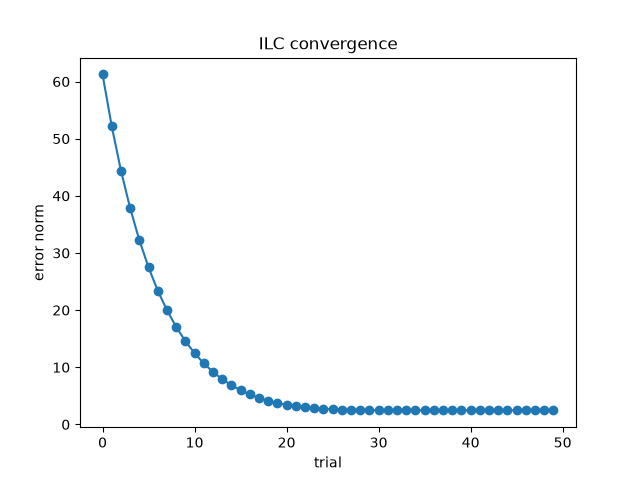
\includegraphics[width=0.7\textwidth]{convergence_plot.png}
  \caption{ILC error norm vs. trial number, 50 trials, gain $=0.2$.}
  \label{fig:convergence}
\end{figure}

\section{Perception and Calibration}

\subsection{ArUco Marker Scheme}

Real joint angles are intended to be recovered from a camera feed using four ArUco markers per side placed on each crank and its base anchor point (\texttt{src/aruco\_track.py}): an anchor pair defines the base-bar orientation in the camera frame, and each crank marker's angle relative to its anchor, minus the base-bar rotation, gives $\theta_i$.

\subsection{Synthetic Validation}

\texttt{notebooks/vision.ipynb} validates the angle-extraction math against synthetic (non-camera) pixel coordinates in three cases: anchors level with the camera frame, the whole rig rotated $30^\circ$ in-frame, and a missing marker (confirmed to degrade gracefully to \texttt{None} rather than crashing).

\subsection{Physical Calibration Status}

Physical ArUco markers (30~mm anchors, 15~mm crank markers, plus a spare end-effector marker) have been generated and printed (\texttt{markers/}).

\todo[inline]{Mount printed ArUco markers on the physical rig, capture calibration data, and populate \texttt{THETA\_OFFSET\_L}/\texttt{THETA\_OFFSET\_R} in \texttt{config.toml} (currently both $0.0$, uninitialized).}

\section{Hardware Build Status}

As of this report, the physical mechanism has been fully assembled: frame, both proximal servos, all pivot bearings, and 3D-printed brackets/couplers are mounted. No electrical or vision calibration has been run on the assembled hardware yet.

\section{Sim-to-Real Comparison}

\todo[inline]{Entire section pending. Requires capturing real joint angle offsets via the ArUco pipeline (Section 6) against simulated/commanded angles -- not done. Once collected: compare simulated ILC tracking (Section 5.2) against measured tracking error on the physical rig, quantify offset correction needed, re-evaluate whether simulated dynamics (Section 4) match observed behavior. No numbers reported here to avoid presenting placeholder/estimated values as measured data.}

\bibliographystyle{ieeetr}
\bibliography{references}

\listoftodos[Open Issues / Not Yet Done]

\end{document}
